\section{Sviluppi futuri}

Per quanto riguarda \textbf{Random Forest}, poiché l'algoritmo offre la 
possibilità di misurare l’importanza della variabile predittore, uno sviluppo 
futuro potrebbe essere utilizzare l'importanza delle variabili, mostrata nella 
figura \ref{fig:rf_importance}, per classificare l'utilità delle variabili, ed 
utilizzare solo le più importanti come feature del modello. 

\begin{figure}[H]
	\centering
	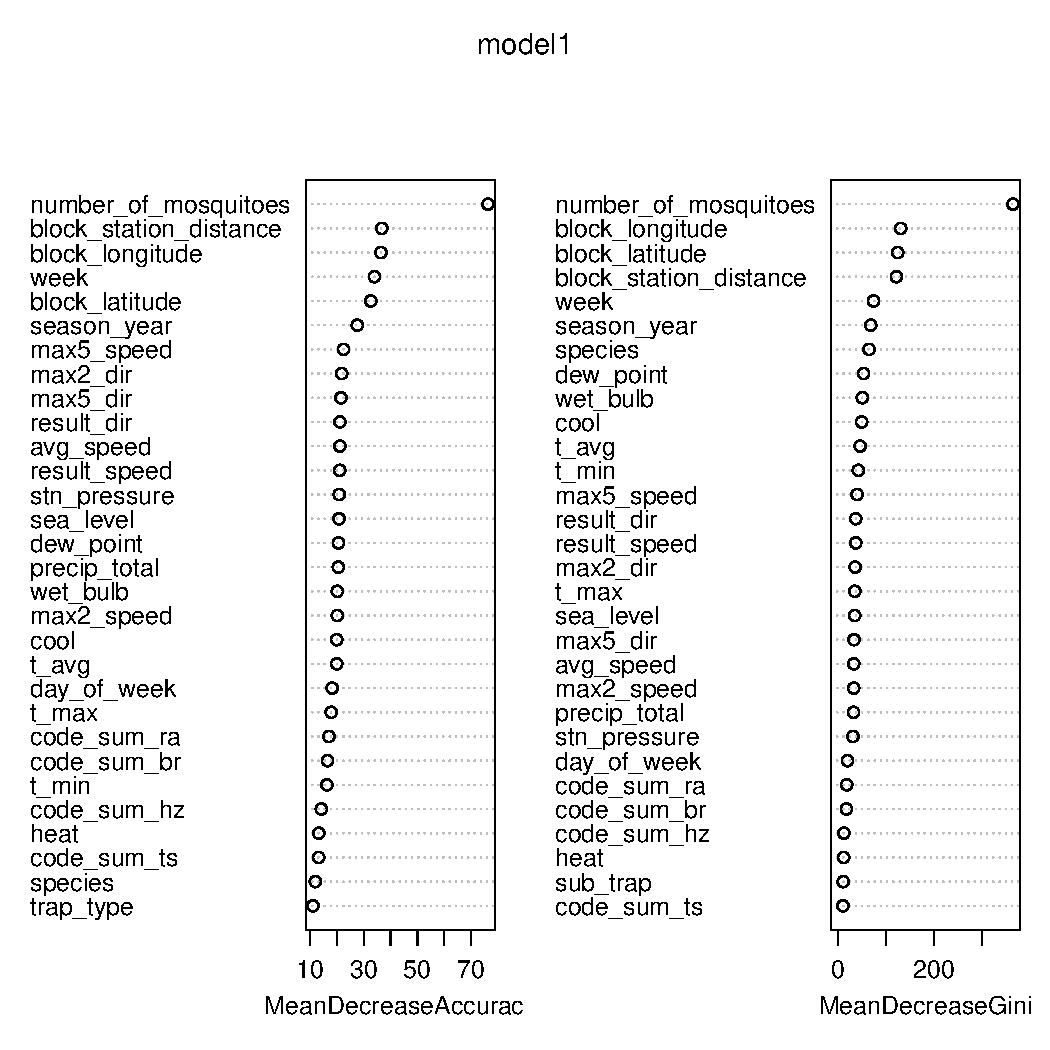
\includegraphics[width=0.6\columnwidth]{images/ml/random_forest/HoldoutRF/model_importance}
	\caption{Random Forest Importance}
	\label{fig:rf_importance}
\end{figure}

